\documentclass[border=4pt]{standalone}
\usepackage{xcolor,amsmath,ctex,tikz,lmodern}
\usetikzlibrary{backgrounds,fit,calc,positioning}
\usetikzlibrary{shapes.geometric,shapes.misc}
\begin{document}
	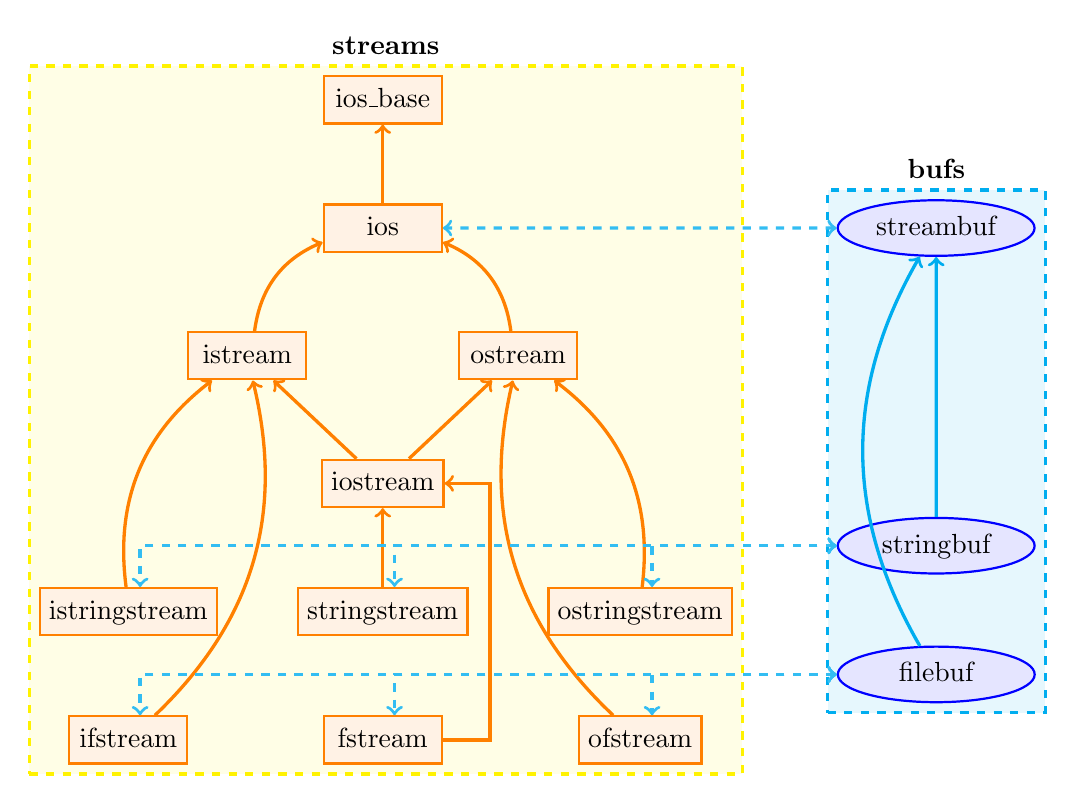
\begin{tikzpicture}[scale=1.5,
		stream/.style={
			text height=1.5ex,text depth=.25ex,
			rectangle,
			minimum width =15mm,
			minimum height= 6mm,
			thick,
			draw=orange,
			fill=orange!10,
			font=\rmfamily
		},
		streambuf/.style={
			text height=1.5ex,text depth=.25ex,
			ellipse,
			minimum width =25mm,
			minimum height= 6mm,
			thick,
			draw=blue,
			fill=blue!10,
			font=\rmfamily
		},
		null/.style={
			minimum width =15mm,
			minimum height= 6mm
		},
		link/.style={
			->,color=orange,very thick
		},
		relate/.style={
			<->,color=cyan!80,dashed,very thick
		}
		]
		\begin{scope}
			\node[stream] (iosbase) {ios\_base};
			\node[stream,below=of iosbase] (ios) {ios}
			edge [link] (iosbase);
			\node[null,below=of ios] (null1) {};
			\node[stream,left =of null1,xshift= 8mm] (istream) {istream}
			edge [link,bend left]  (ios);
			\node[stream,right=of null1,xshift=-8mm] (ostream) {ostream}
			edge [link,bend right] (ios);
			\node[stream,below=of null1] (iostream) {iostream}
			edge [link] (istream)
			edge [link] (ostream);
			\node[stream,below=of iostream] (stringstream) {stringstream}
			edge [link] (iostream);
			\node[stream,left =of stringstream] (istringstream) {istringstream}
			edge [link,bend left]  (istream);
			\node[stream,right=of stringstream] (ostringstream) {ostringstream}
			edge [link,bend right] (ostream);
			\node[stream,below=of stringstream] (fstream) {fstream};
			\draw[link] (fstream.east) -- ++(4mm,0) |- (iostream.east);
			\node[stream,below=of istringstream] (ifstream) {ifstream}
			edge [link,bend right] (istream);
			\node[stream,below=of ostringstream] (ofstream) {ofstream}
			edge [link,bend left]  (ostream);
			\node[streambuf,right=of ios      ,xshift= 40mm] (streambuf) {streambuf}
			edge [relate] (ios);
			\node[streambuf,below=of streambuf,yshift=-23mm] (stringbuf) {stringbuf}
			edge [link,color=cyan] (streambuf);
			\draw [relate] (stringbuf) -| ($(istringstream.north) + (.1,0)$);
			\draw [relate] (stringbuf) -| ($(ostringstream.north) + (.1,0)$);
			\draw [relate] (stringbuf) -| ($ (stringstream.north) + (.1,0)$);
			\node[streambuf,below=of stringbuf,yshift=  1mm] (filebuf) {filebuf}
			edge [link,color=cyan,bend left] (streambuf);
			\draw [relate] (filebuf) -| ($(ifstream.north) + (.1,0)$);
			\draw [relate] (filebuf) -| ($(ofstream.north) + (.1,0)$);
			\draw [relate] (filebuf) -| ($ (fstream.north) + (.1,0)$);
		\end{scope}
		\begin{scope}[on background layer]
			\node[
			fill=yellow!10,very thick,dashed,draw=yellow,
			label=north:{\textbf{streams}},
			fit=(iosbase) (ifstream) (ofstream) (istringstream) (ostringstream)
			] (streams) {};
			\node[
			fill=cyan!10,very thick,dashed,draw=cyan,
			label=north:{\textbf{bufs}},
			fit=(streambuf) (stringbuf) (filebuf)
			] (bufs) {};
		\end{scope}
	\end{tikzpicture}
\end{document}